
\documentclass[12pt, a4paper]{article}  

%%%%%%%%%% Математика %%%%%%%%%%
\usepackage{amsmath,amsfonts,amssymb,amsthm,mathtools} 
%\mathtoolsset{showonlyrefs=true}  % Показывать номера только у тех формул, на которые есть \eqref{} в тексте.
%\usepackage{leqno} % Нумерация формул слева


%%%%%%%%%%%%%%% Шрифты %%%%%%%%%%%
\usepackage{fontspec}         % пакет для подгрузки шрифтов
\setmainfont{Arial}   % задаёт основной шрифт документа

\defaultfontfeatures{Mapping=tex-text}

% why do we need \newfontfamily:
% http://tex.stackexchange.com/questions/91507/
\newfontfamily{\cyrillicfonttt}{Arial}
\newfontfamily{\cyrillicfont}{Arial}
\newfontfamily{\cyrillicfontsf}{Arial}
% Грубо говоря иногда polyglossia начинает балбесничать и не видит структуры кириллических шрифтов. Эти трое бравых парней спасают ситуацию и доопределяют те куски, которые Тех не увидел.

\usepackage{unicode-math}     % пакет для установки математического шрифта
\setmathfont{Asana Math}      % шрифт для математики
% \setmathfont[math-style=ISO]{Asana Math}
% Можно делать смену начертания с помощью разных стилей

% Конкретный символ из конкретного шрифта
% \setmathfont[range=\int]{Neo Euler}


\usepackage{polyglossia}      % Пакет, который позволяет подгружать русские буквы
\setdefaultlanguage{russian}  % Основной язык документа
\setotherlanguage{english}    % Второстепенный язык документа

\author{Мартыненко Маргарита} 
\title{Уютная домашка № 2}
\date{\today}

               







\begin{document}



\maketitle
\newpage


\section{Задание 1} 


 \begin{figure}[h!]
\begin{minipage}[H]{0.3\linewidth} 
\center 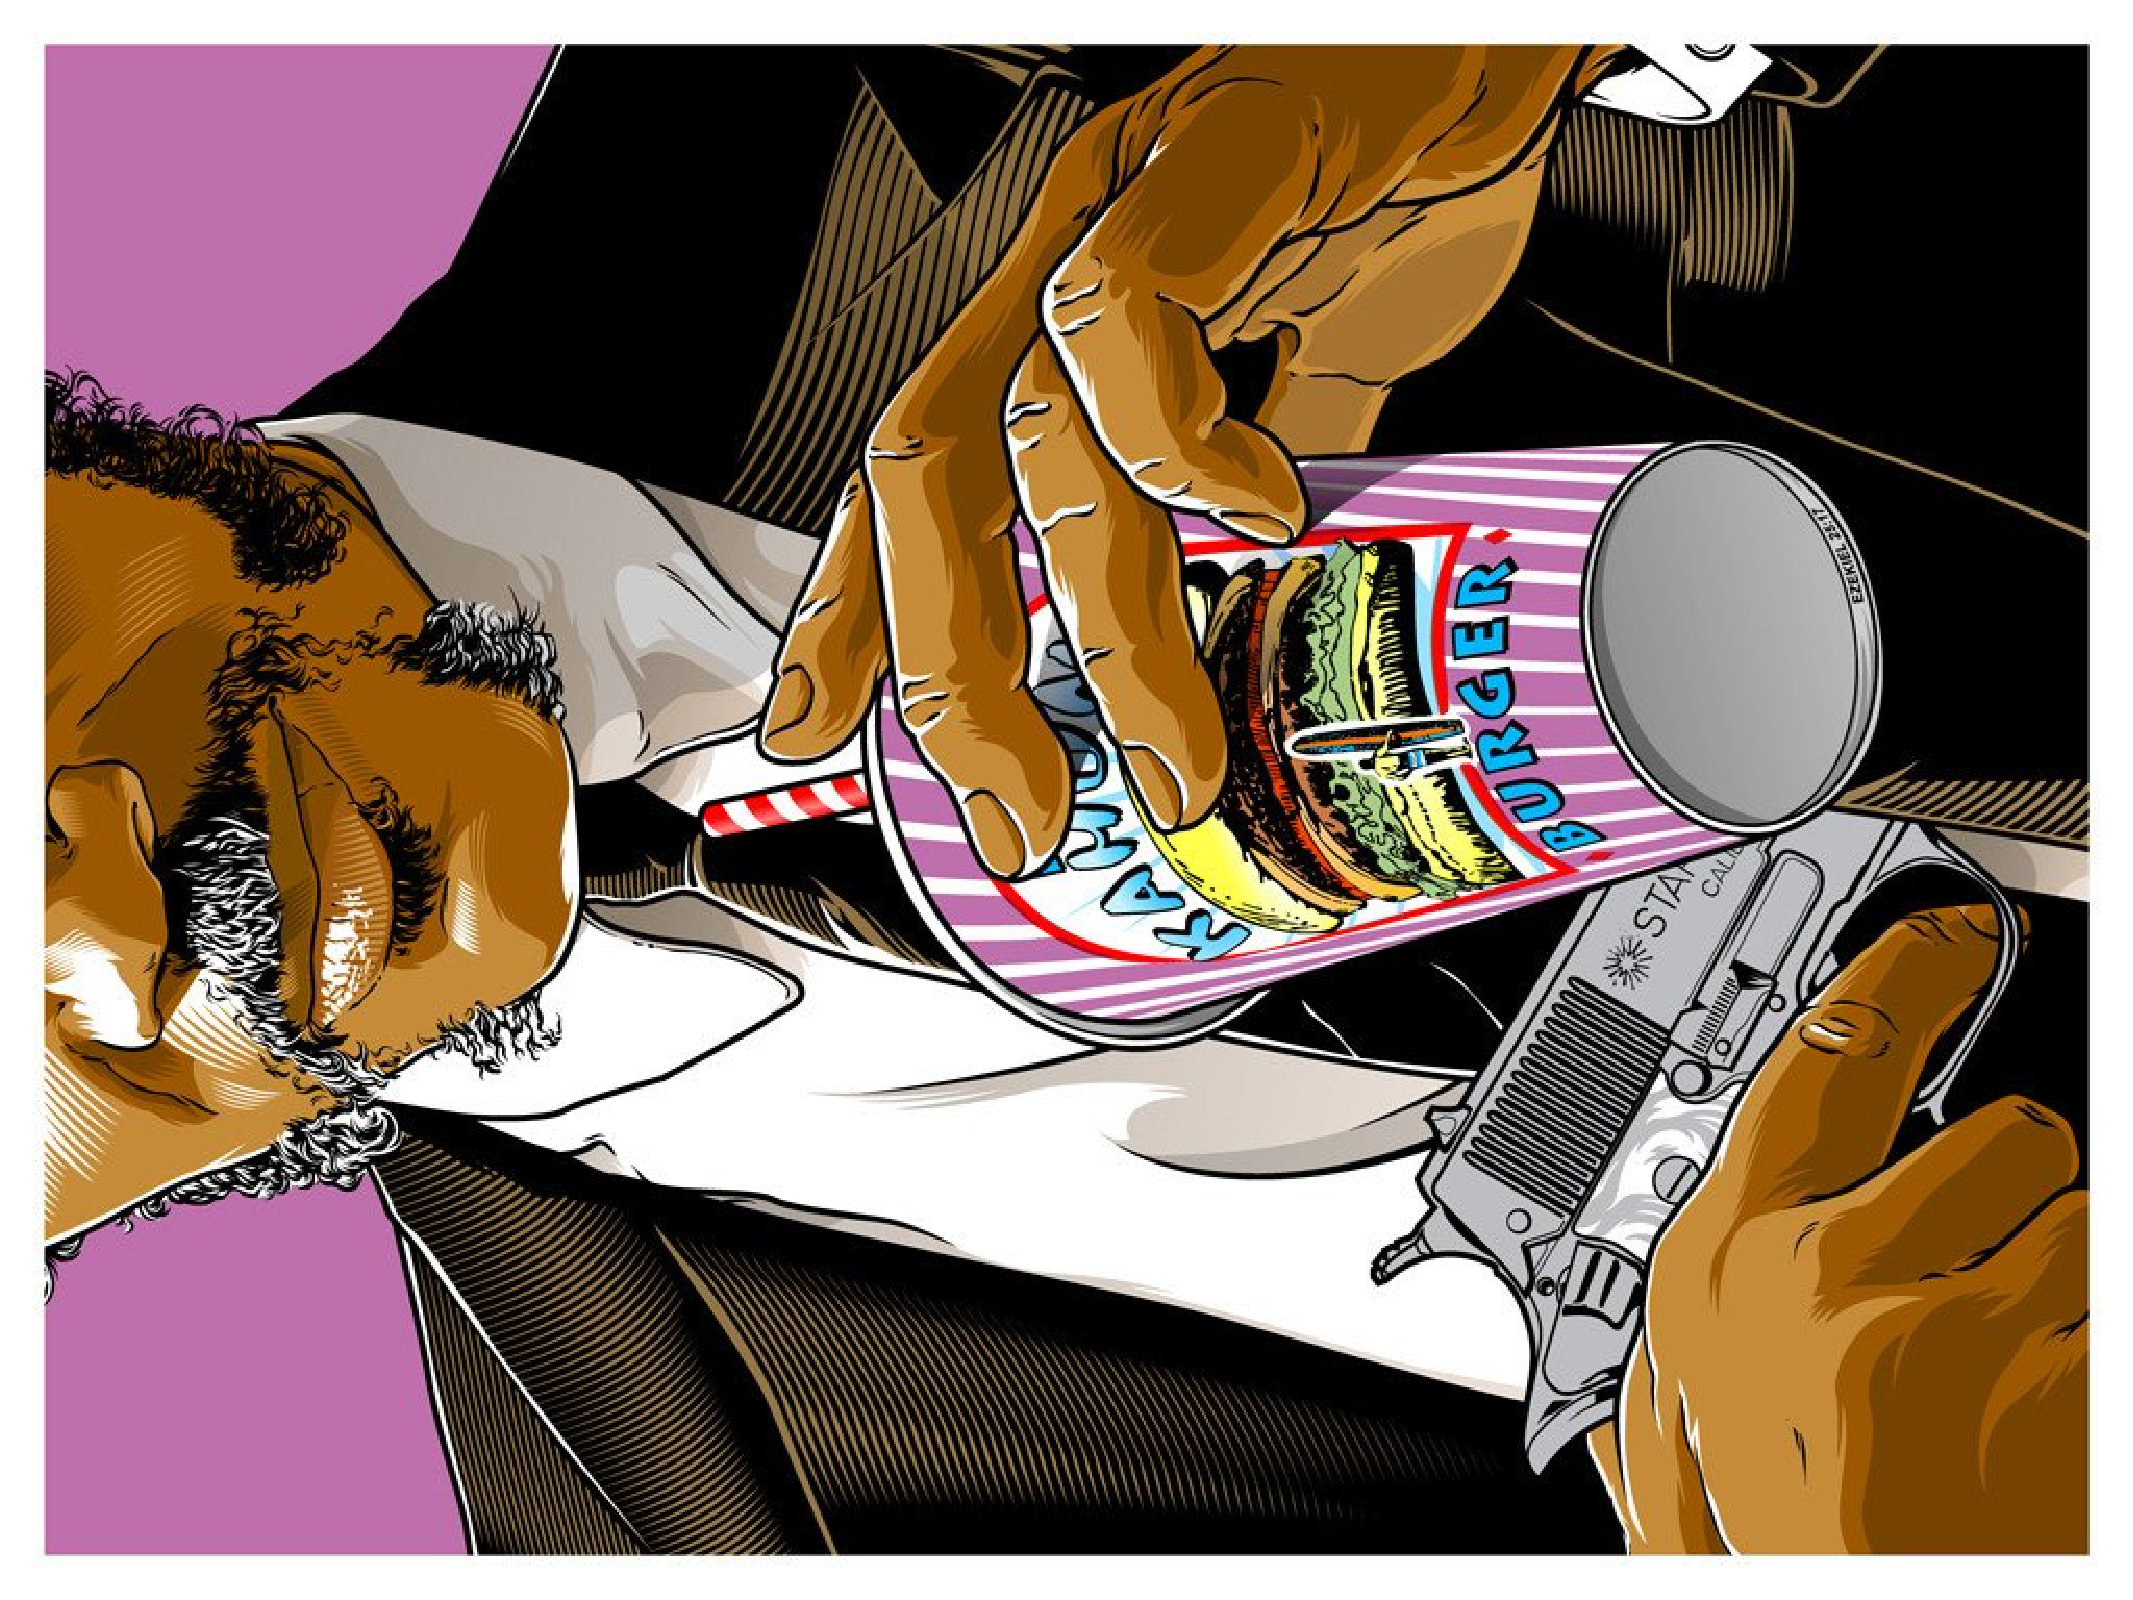
\includegraphics[height=4cm,width=5cm,angle = 270]{pop1.pdf}
\end{minipage}
\begin{minipage}[H]{0.3\linewidth} 
\center  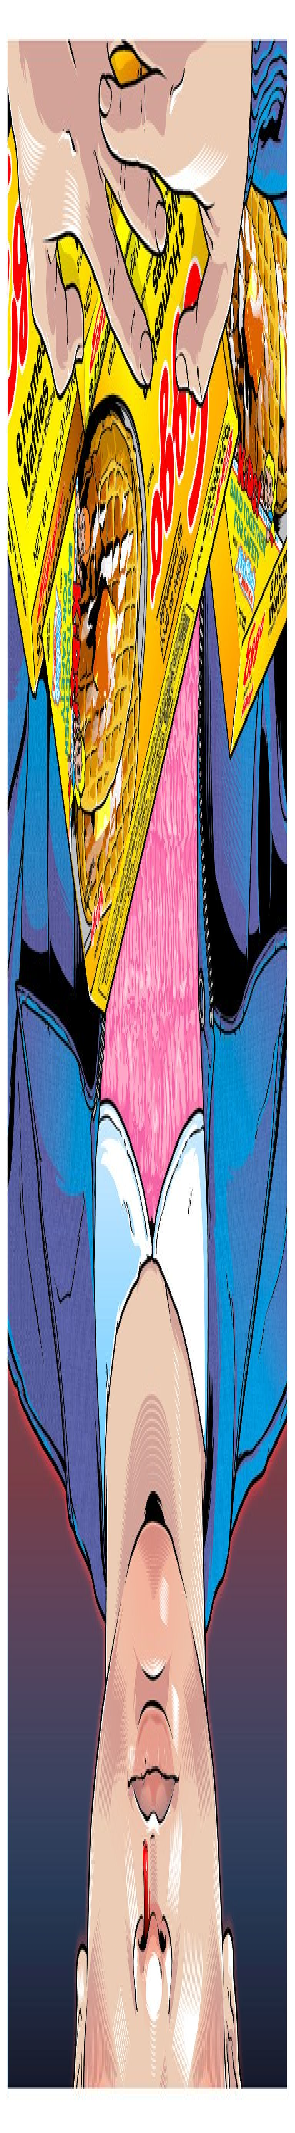
\includegraphics[height=5cm,width=4cm,angle = 180]{pop2.pdf}
\end{minipage}
\begin{minipage}[H]{0.3\linewidth} 
\center  
\includegraphics[height=5cm,width=4cm]{pop3.pdf}
\end{minipage}
\vfil
\begin{minipage}[H]{0.3\linewidth} 
\center  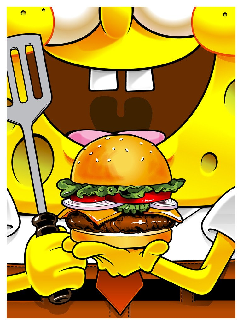
\includegraphics[height=5cm,width=4cm]{pop8.pdf}
\end{minipage}
\begin{minipage}[H]{0.3\linewidth} 
\center  \includegraphics[height=5cm,width=4cm]{pop5.pdf}
\end{minipage}
\begin{minipage}[H]{0.3\linewidth} 
\center  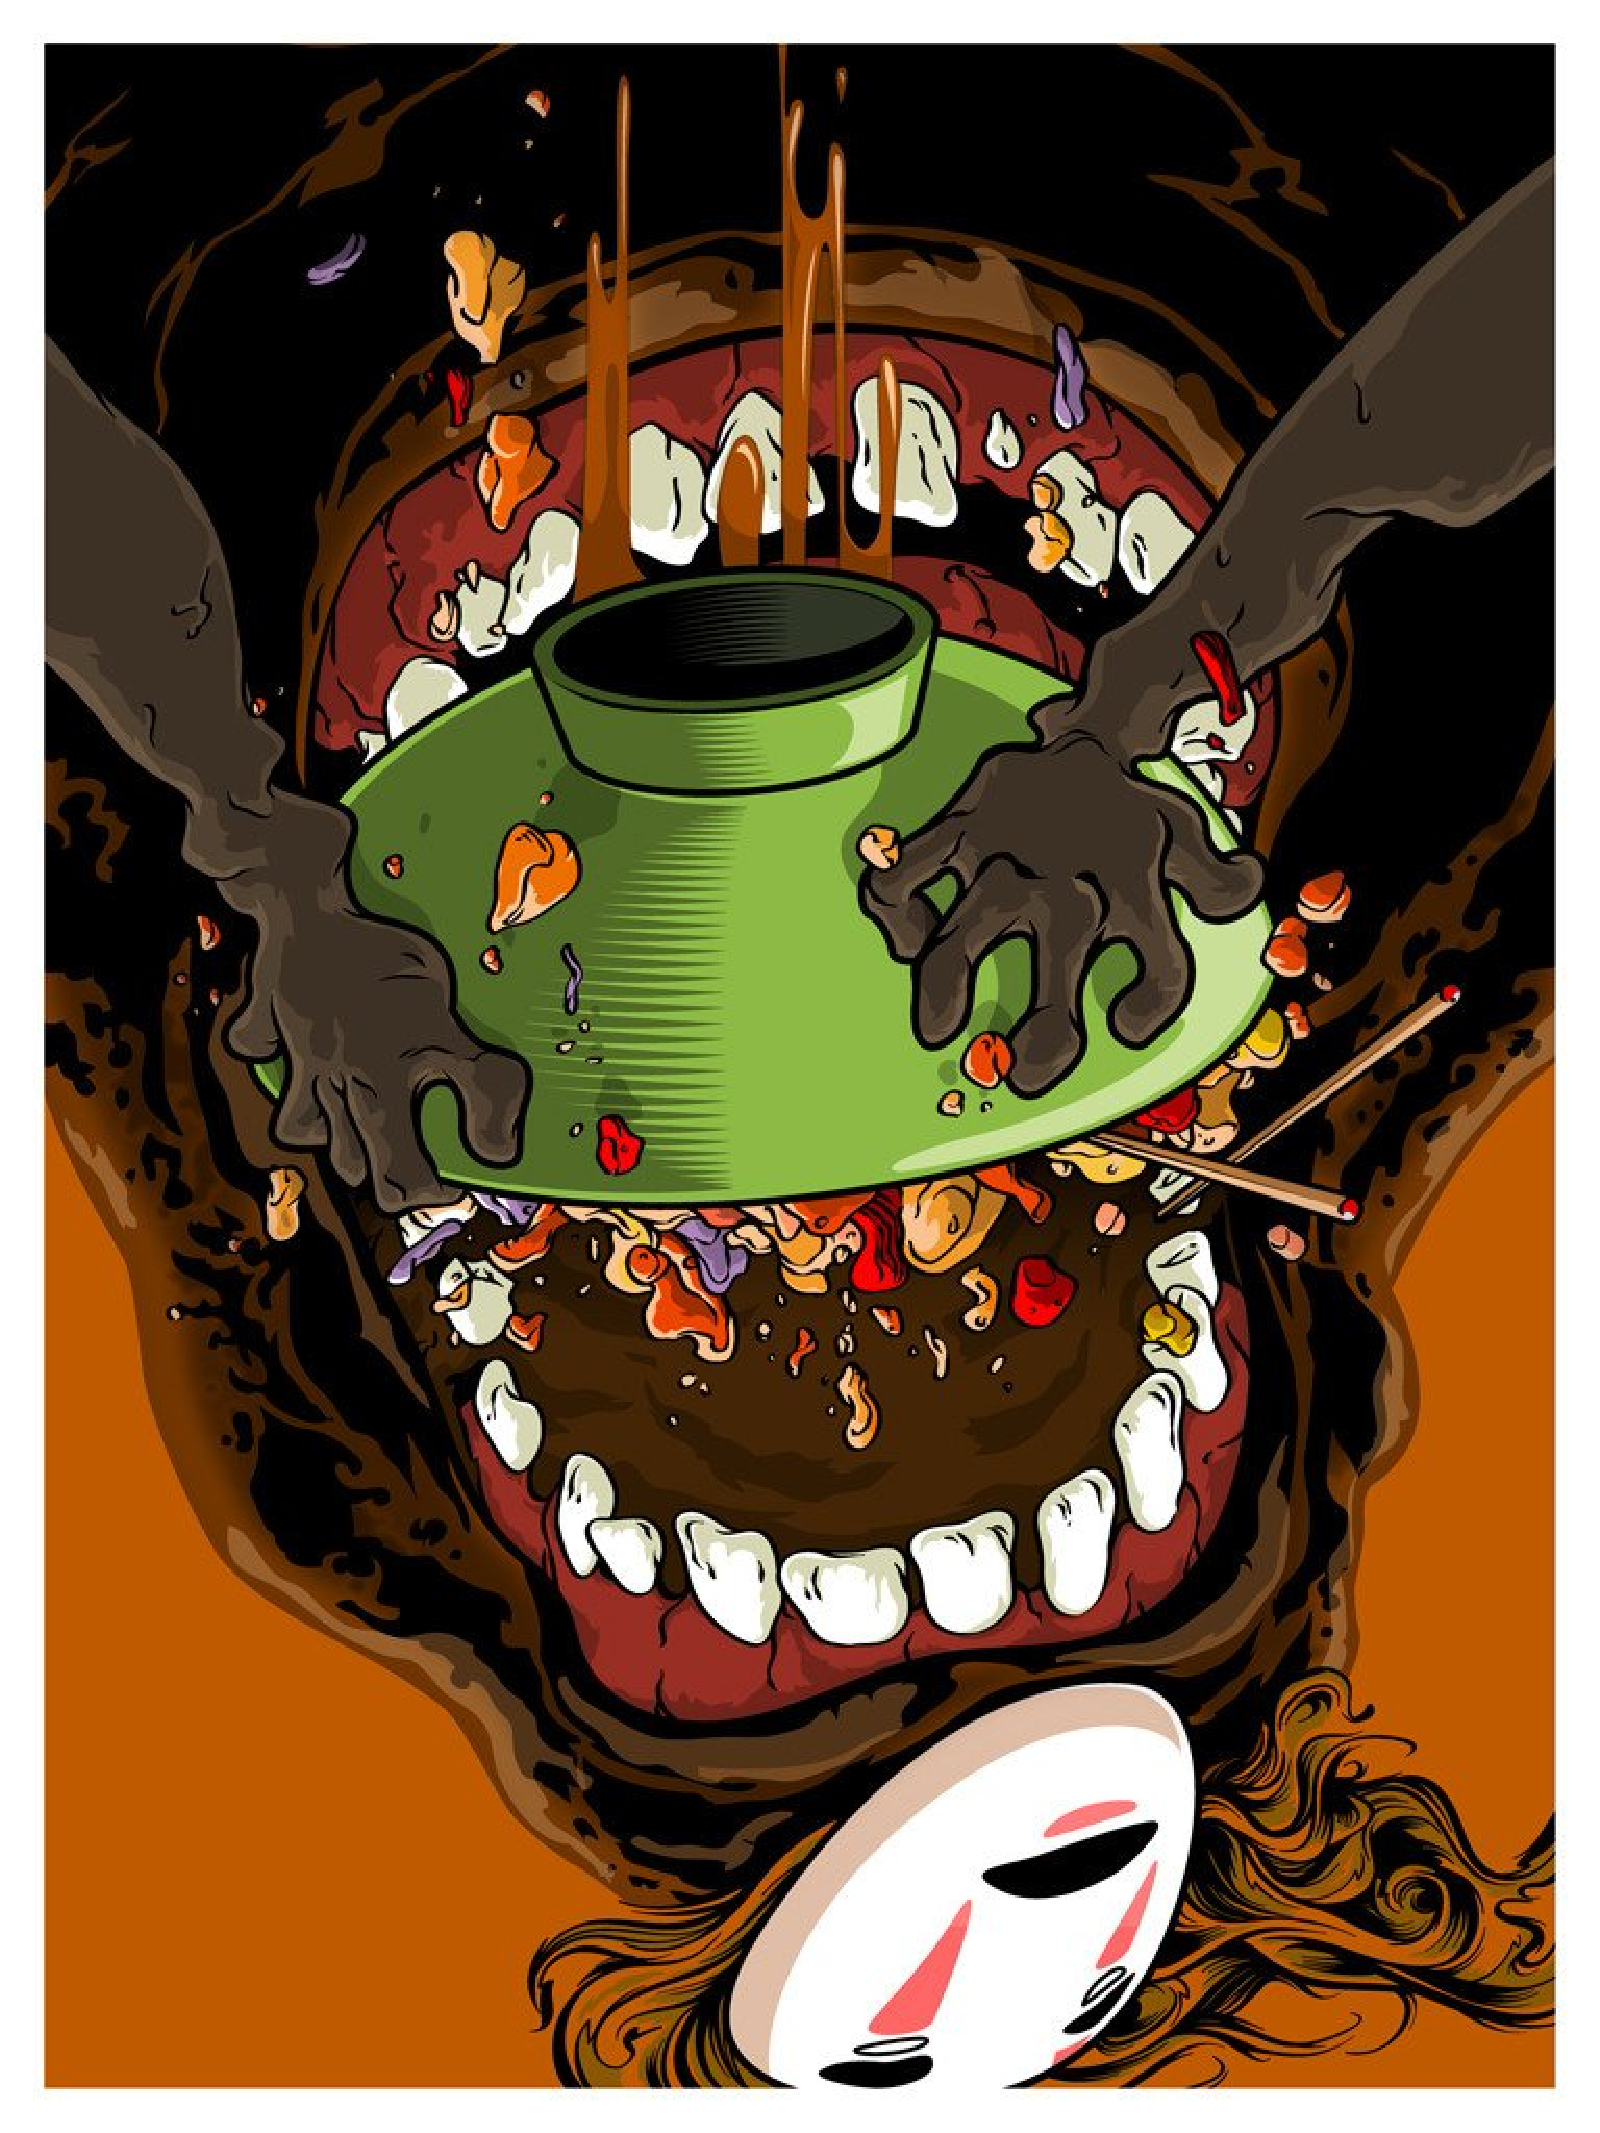
\includegraphics[height=5cm,width=4cm,angle = 180]{pop6.pdf}
\end{minipage}
\caption{Это что: поп-арт?!}
\end{figure}





\end{document}

